\begin{center}
    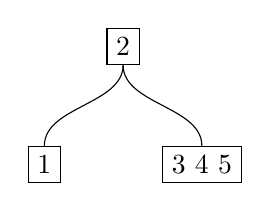
\begin{tikzpicture}[
       edge from parent path=
    {(\tikzparentnode.south) .. controls +(0,-.5) and +(0,.5)
                             .. (\tikzchildnode.north)},
    level 1/.style={sibling distance=2cm},                         
   every node/.style={draw},
   label distance=-1mm]
   
\node {2}
    child {node {1}}   
    child {node {3 4 5}
    };

\end{tikzpicture}
\end{center}

\begin{center}
    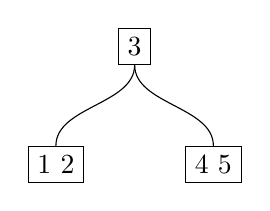
\begin{tikzpicture}[
       edge from parent path=
    {(\tikzparentnode.south) .. controls +(0,-.5) and +(0,.5)
                             .. (\tikzchildnode.north)},
    level 1/.style={sibling distance=2cm},                       
   every node/.style={draw},
   label distance=-1mm]
   
\node {3}
    child {node {1 2}}   
    child {node {4 5}
    };

\end{tikzpicture}
\end{center}

\begin{center}
    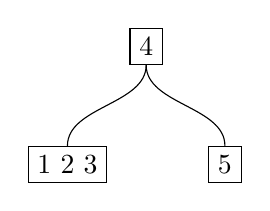
\begin{tikzpicture}[
       edge from parent path=
    {(\tikzparentnode.south) .. controls +(0,-.5) and +(0,.5)
                             .. (\tikzchildnode.north)},
    level 1/.style={sibling distance=2cm},                        
   every node/.style={draw},
   label distance=-1mm]
   
\node {4}
    child {node {1 2 3}}   
    child {node {5}
    };

\end{tikzpicture}
\end{center}

\begin{center}
    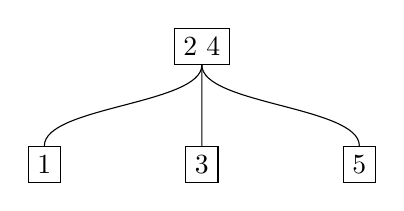
\begin{tikzpicture}[
       edge from parent path=
    {(\tikzparentnode.south) .. controls +(0,-.5) and +(0,.5)
                             .. (\tikzchildnode.north)},
    level 1/.style={sibling distance=2cm},                        
   every node/.style={draw},
   label distance=-1mm]
   
\node {2 4}
    child {node {1}}   
    child {node {3}}
    child {node {5}
    };

\end{tikzpicture}
\end{center}
